%\documentclass[10pt, twocolumn]{article}
\documentclass[twocolumn,showpacs,preprintnumbers,amsmath,amssymb,prd]{revtex4}
%\documentclass[11 pt,preprint,preprintnumbers,amsmath,amssymb, prd]{revtex4}

% Preamble adapted from Surjeet Rajendran

\usepackage{latexsym}
\usepackage{amssymb}
\usepackage{epsfig,amsmath,graphics}
\usepackage{epstopdf}
\usepackage{verbatim}
\usepackage{wasysym}
\usepackage{hyperref}
\usepackage{feynmp-auto} % feynman diagrams
%\usepackage{subfig}
\usepackage[utf8]{inputenc}
\usepackage{xpatch}
\usepackage{xcolor}
\hypersetup{
    colorlinks,
    linkcolor={red!80!black},
    citecolor={green!60!black},
    urlcolor={blue!60!black}
}
\usepackage{appendix}

\newcommand{\OO}{\mathcal{O}}
\newcommand{\LL}{\mathcal{L}}
\newcommand{\HH}{\mathcal{H}}

\newcommand{\GeV}{\text{GeV}}
\newcommand{\MeV}{\text{MeV}}
\newcommand{\keV}{\text{keV}}
\newcommand{\rad}{\text{rad}}
\newcommand{\cm}{\text{cm}}
\newcommand{\angstrom}{\buildrel _{\circ} \over {\mathrm{A}}}
\newcommand{\pslash}{p\hspace{-0.070in}/\,}
\newcommand{\Mpl}{M_{\text{pl}}}
\newcommand{\ket}[1]{\ensuremath{\left|#1\right>}}
\newcommand{\bra}[1]{\ensuremath{\left<#1\right|}}
\newcommand{\braket}[2]{\ensuremath{\left<#1|#2\right>}}
%Large Parentheses
\def\r{\right)}
\def\l{\left(}

\begin{document}

\title{White Dwarfs as Dark Matter Detectors}


\author{Ryan Janish}
\affiliation{Berkeley Center for Theoretical Physics, Department of Physics,
University of California, Berkeley, CA 94720, USA}

\author{Vijay Narayan}
\affiliation{Berkeley Center for Theoretical Physics, Department of Physics,
University of California, Berkeley, CA 94720, USA}

\author{Paul Riggins}
\affiliation{Berkeley Center for Theoretical Physics, Department of Physics,
University of California, Berkeley, CA 94720, USA}

\begin{abstract}

White dwarfs can serve as detectors for ultra-heavy dark matter states which interact to trigger type Ia supernovae. This was originally proposed in \cite{Graham:2015apa} and used to  place bounds on primordial black holes. In this paper we extend the capability of white dwarf detectors to candidates with non-gravitational couplings, focusing on dark matter transits and collisions within the white dwarf. In particular, we provide a detailed analysis of the explosiveness for any heating mechanism in the white dwarf which releases high-energy standard model particles. We apply this mechanism to constrain Q-ball dark matter \textcolor{blue}{and model of dark nuclei} in regions of parameter space fundamentally inaccessible to terrestrial-based experiments.

\end{abstract}
\maketitle


\section{Introduction}
\label{sec:Introduction}

The detection of ultra-heavy dark matter (DM) is an open problem which will ultimately require a confluence of astrophysical probes. For instance, DM masses above $\sim 10^{22} ~\GeV$ will register fewer than 1 event per year in a typical terrestrial detector of size $\sim (100 ~\text{m})^2$. Furthermore, the lack of conclusive signatures on a variety of experimental fronts has led many to seriously consider DM candidates far above the weak scale and their potential signatures \textcolor{blue}{cite people}. One possibility proposed by \cite{Graham:2015apa} is that ultra-heavy DM can trigger supernovae in sub-Chandrasekhar white dwarf (WD) stars by inducing runaway fusion.  In this regard, white dwarfs can serve as detectors for ultra-heavy DM states.

White dwarfs are particularly suited to this task, as they are more susceptible to runaway fusion than are main-sequence stars. Runaway fusion requires that two criteria be met: a region within the star must be hot enough to support exothermic fusion reactions, and the rate at which energy is released by these reactions must dominate any cooling mechanisms that drain energy from the fusing region.  The stellar medium of a WD has fewer cooling mechanisms available than does a non-degenerate star - WD cooling relies on thermal diffusion whereas main-sequence stars can also cool via thermal expansion.  This is suppressed in a WD since its pressure is determined by electron degeneracy and is thus independent of temperature. The remaining primary cooling mechanism, diffusion, becomes less important over longer length scales and can be overcome by sufficiently heating a large enough region of the WD.

The necessary trigger for runaway fusion was initially computed in \cite{Woosley} and subsequently implemented in \cite{Graham:2015apa} to constrain primordial black holes, which can ignite WD stars via gravitational dynamical friction.  In addition, the authors of \cite{Graham:2015apa} identify several other heating mechanisms involving DM which may be constrained in a similar manner.  \textcolor{blue}{Some of these have been explored in follow-up works...citations, citations.}  In this work, we extend their analysis to DM candidates with generic non-gravitational couplings, focusing on DM transits through the WD and DM-DM collisions within the WD which release energy in the form of standard model (SM) particles. More generally, we provide a detailed analysis of the explosive power and resulting constraints on any DM with interactions of this sort.

Concrete examples of DM candidates with interactions of this type include baryonic Q-balls found in supersymmetric extensions of the SM and \textcolor{blue}{dark nuclei with high-order couplings to the SM.} We are able to constrain these models in regions of parameter space fundamentally inaccessible to terrestrial experiments. However, it is important to note that any such DM constraints are by nature complimentary to terrestrial ones - it is more massive DM that is likely to trigger supernovae, and also more massive DM that have sufficiently low flux on Earth. What allows the WD to be effective in this regime is its enhanced surface area $\sim (4000 ~\text{km})^2$ and exceptionally long lifetime $\sim \text{Gyr}$. In this sense, the WD is a large ``space-time volume" detector. \textcolor{blue}{We also have a ``flux is too low" limit...should we include here?}

\textcolor{blue}{Other ignition sources exist (i.e., detector backgrounds). How does this limit our constraints? Discuss the specific tests we apply (WD lifetime, SN rate) to derive our constraints.} \textcolor{red}{Possible long term addition: improve constraints by using non-type IA sn rate instead of total rate. Should talk with SN people first.}

We begin in Section~\ref{sec:Review} by reviewing the explosion mechanism in a WD. In Section~\ref{sec:DMexplode}, we parametrize the properties of DM necessary to trigger explosions through non-gravitational interactions in the case of a DM transit or collision in the star. The precise explosive power will be determined by a heating length, which is computed in Section~\ref{sec:HeatingLength} for different possible interactions. Following this general discussion, we apply the WD detector to place constraints on ultra-heavy dark matter in Section~\ref{sec:Constraints}, and apply these constraints in Section~\ref{sec:ConcreteExamples} to Q-balls and dark nuclei as concrete examples. We conclude in Section~\ref{sec:discussion}.

\section{White Dwarf Runaway Fusion}
\label{sec:Review}
In a WD, the \emph{fusion temperature} $T_f$ is a constant set by the energy required for ions to overcome their mutual Coulomb barriers $T_f \sim \MeV$. WD cooling is set by the thermal diffusivity of photons and degenerate electrons. The two species dominate the cooling at different stellar densities, as determined precisely in \cite{Woosley}. Note that for a heated region of size $R$, this cooling rate scales as $R^{-2}$ while the fusion rate scales as $R^{-3}$. Thus there is a critical \emph{trigger size} $\lambda_T$ below which diffusive cooling dominates the thermal evolution of a temperature peak, and above which the liberated fusion energy dominates \cite{Woosley}. Therefore, a region with temperature greater than $T_f$ and size greater than $\lambda_T$ in a given WD will launch a runaway fusion chain-reaction and result in a type Ia supernova. The numerical value of $\lambda_T$ is highly sensitive to the WD density and has been analytically scaled for varying WD masses in \cite{Graham:2015apa}. As in \cite{Graham:2015apa}, we restrict our attention to carbon-oxygen WDs in the upper mass range $0.7 - 1.4 ~M_{\odot}$ which correspond to a number density of nuclei $n_i \sim 10^{29} - 10^{32} ~\cm^{-3}$. Over this range, the trigger size is approximately $\lambda_T \sim 10^{-5} - 10^{-2} ~\text{cm}$.

A general energy deposition event in the WD can be roughly characterized by two parameters: a temperature $T$ and heating length $L$. This energy deposit will eventually take the form of a local peak in the WD temperature profile. We define $T$ to be the characteristic temperature and $L$ the characteristic length scale of this local peak as it initially appears. $L$ is determined by the efficiency with which a given energy deposition mechanism interacts with the stellar medium. To demonstrate the significance of $L$, suppose that kinetic energy were transferred directly to neighboring ions via short-range elastic scatters. These ions would thermalize over their collisional time scale resulting in a heating length $L$ of order the ion mean free path. In the other extreme, suppose that a process produces a large number of electrons with energy just above the Fermi energy.  These electrons have Pauli-suppressed interactions with the medium and will travel a long distance before their energy is scattered and thermalized, resulting in a large $L$ - possibly of order the stellar radius.

We find that a heating event will destroy a given WD as long as the energy density \emph{and} energy deposited are sufficiently large:
\begin{equation}
\label{eq:runaway}
T \gtrsim T_f, ~~~~ L \gtrsim \lambda_T.
\end{equation}
Note that this condition determines if a region of size $L$ and temperature $T$ \emph{immediately} initiates runaway fusion.  Instead, it is more useful to determine whether a given energy deposit will \emph{eventually} initiate runaway fusion. In particular, a heating event that results in $T \gg T_f$ and $L  < \lambda_T$ is perhaps initially dominated by diffusive cooling but can potentially evolve into an ``explosive" temperature profile capable of igniting the star. When diffusion dominates, the thermal evolution will approximately be given by the dilution of the fixed total energy of the initial region over the final volume. Taking this into account, we can express the explosion condition \eqref{eq:runaway} in terms of an excess energy within the temperature peak (rather than the temperature itself):
\begin{equation}
\label{eq:boom}
E \gtrsim n_i T_f \text{max}\{L, \lambda_T\}^3.
\end{equation}
In fact, there is an absolute minimum explosion energy given by
\begin{equation}
E_{\text{boom}} \sim n_i T_f \lambda_T^3 \sim 10^{14} - 10^{21} ~\GeV,
\end{equation}
where the trigger size $\lambda_T$ varies over a range of WD densities. This is plotted in Figure \ref{fig:Eboom}. However, this energy is sufficient only if it thermalizes within the trigger size.  If an energy is deposited on a length scale larger than $\lambda_T$, the explosion energy required is given by \eqref{eq:boom} and may be parametrically larger. Since we are concerned with processes that have a fixed deliverable energy (the energy of the incoming DM), the most explosive processes will be those that result in the most localized heating. As a result, understanding the heating length $L$ for various processes is critical to assessing their explosive potential. This is done in Section~\ref{sec:heatinglength}.

\begin{figure}
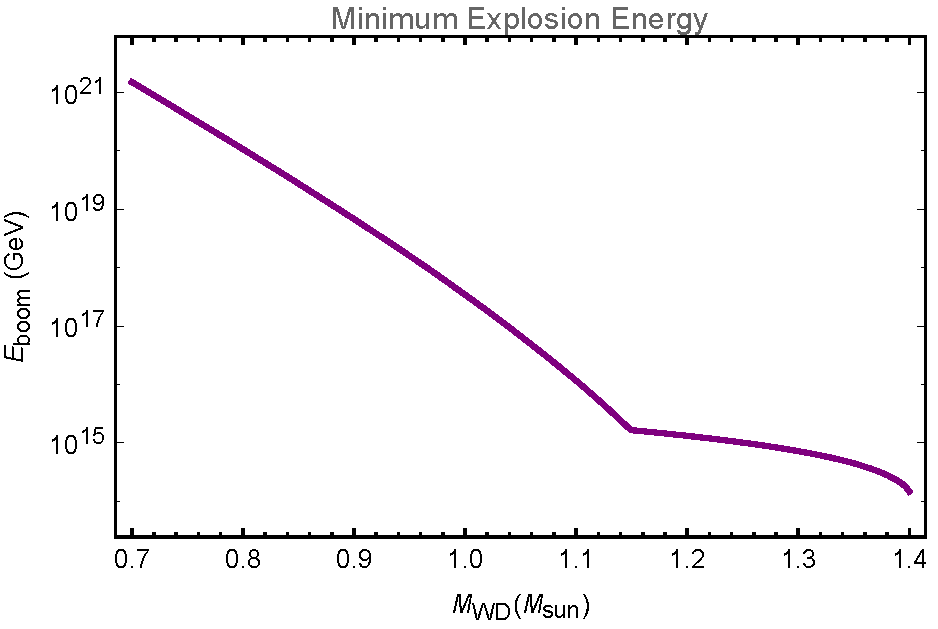
\includegraphics[scale=.45]{Eboom.pdf}
\caption{Minimum energy required to trigger explosion in a WD, based on numerical results for $\lambda_T$ \cite{Woosley}.}
\label{fig:Eboom}
\end{figure}

\section{Dark Matter Explosiveness}
\label{sec:DMexplode}

In this section we parameterize the ability of generic, non-gravitational dark matter interactions to destroy a WD.  We focus on DM-SM and DM-DM interactions, as depicted in Figure \ref{feynman}, which can cause local heating through the release of high-energy SM particles. The former allows stellar heating via \emph{transit} events as the DM continually releases energy while traversing the star, while the latter leads to heating via point-like \emph{collision} events.  Note that these collisions are not necessarily particle-antiparticle annihilations but may be of a more complicated nature, such as the collisions of heavy nuclei.  The heating mechanism and event rates will be parametrically different for DM transits and collision, and thus we treat of these cases separately. 

\begin{figure}
\label{feynman}
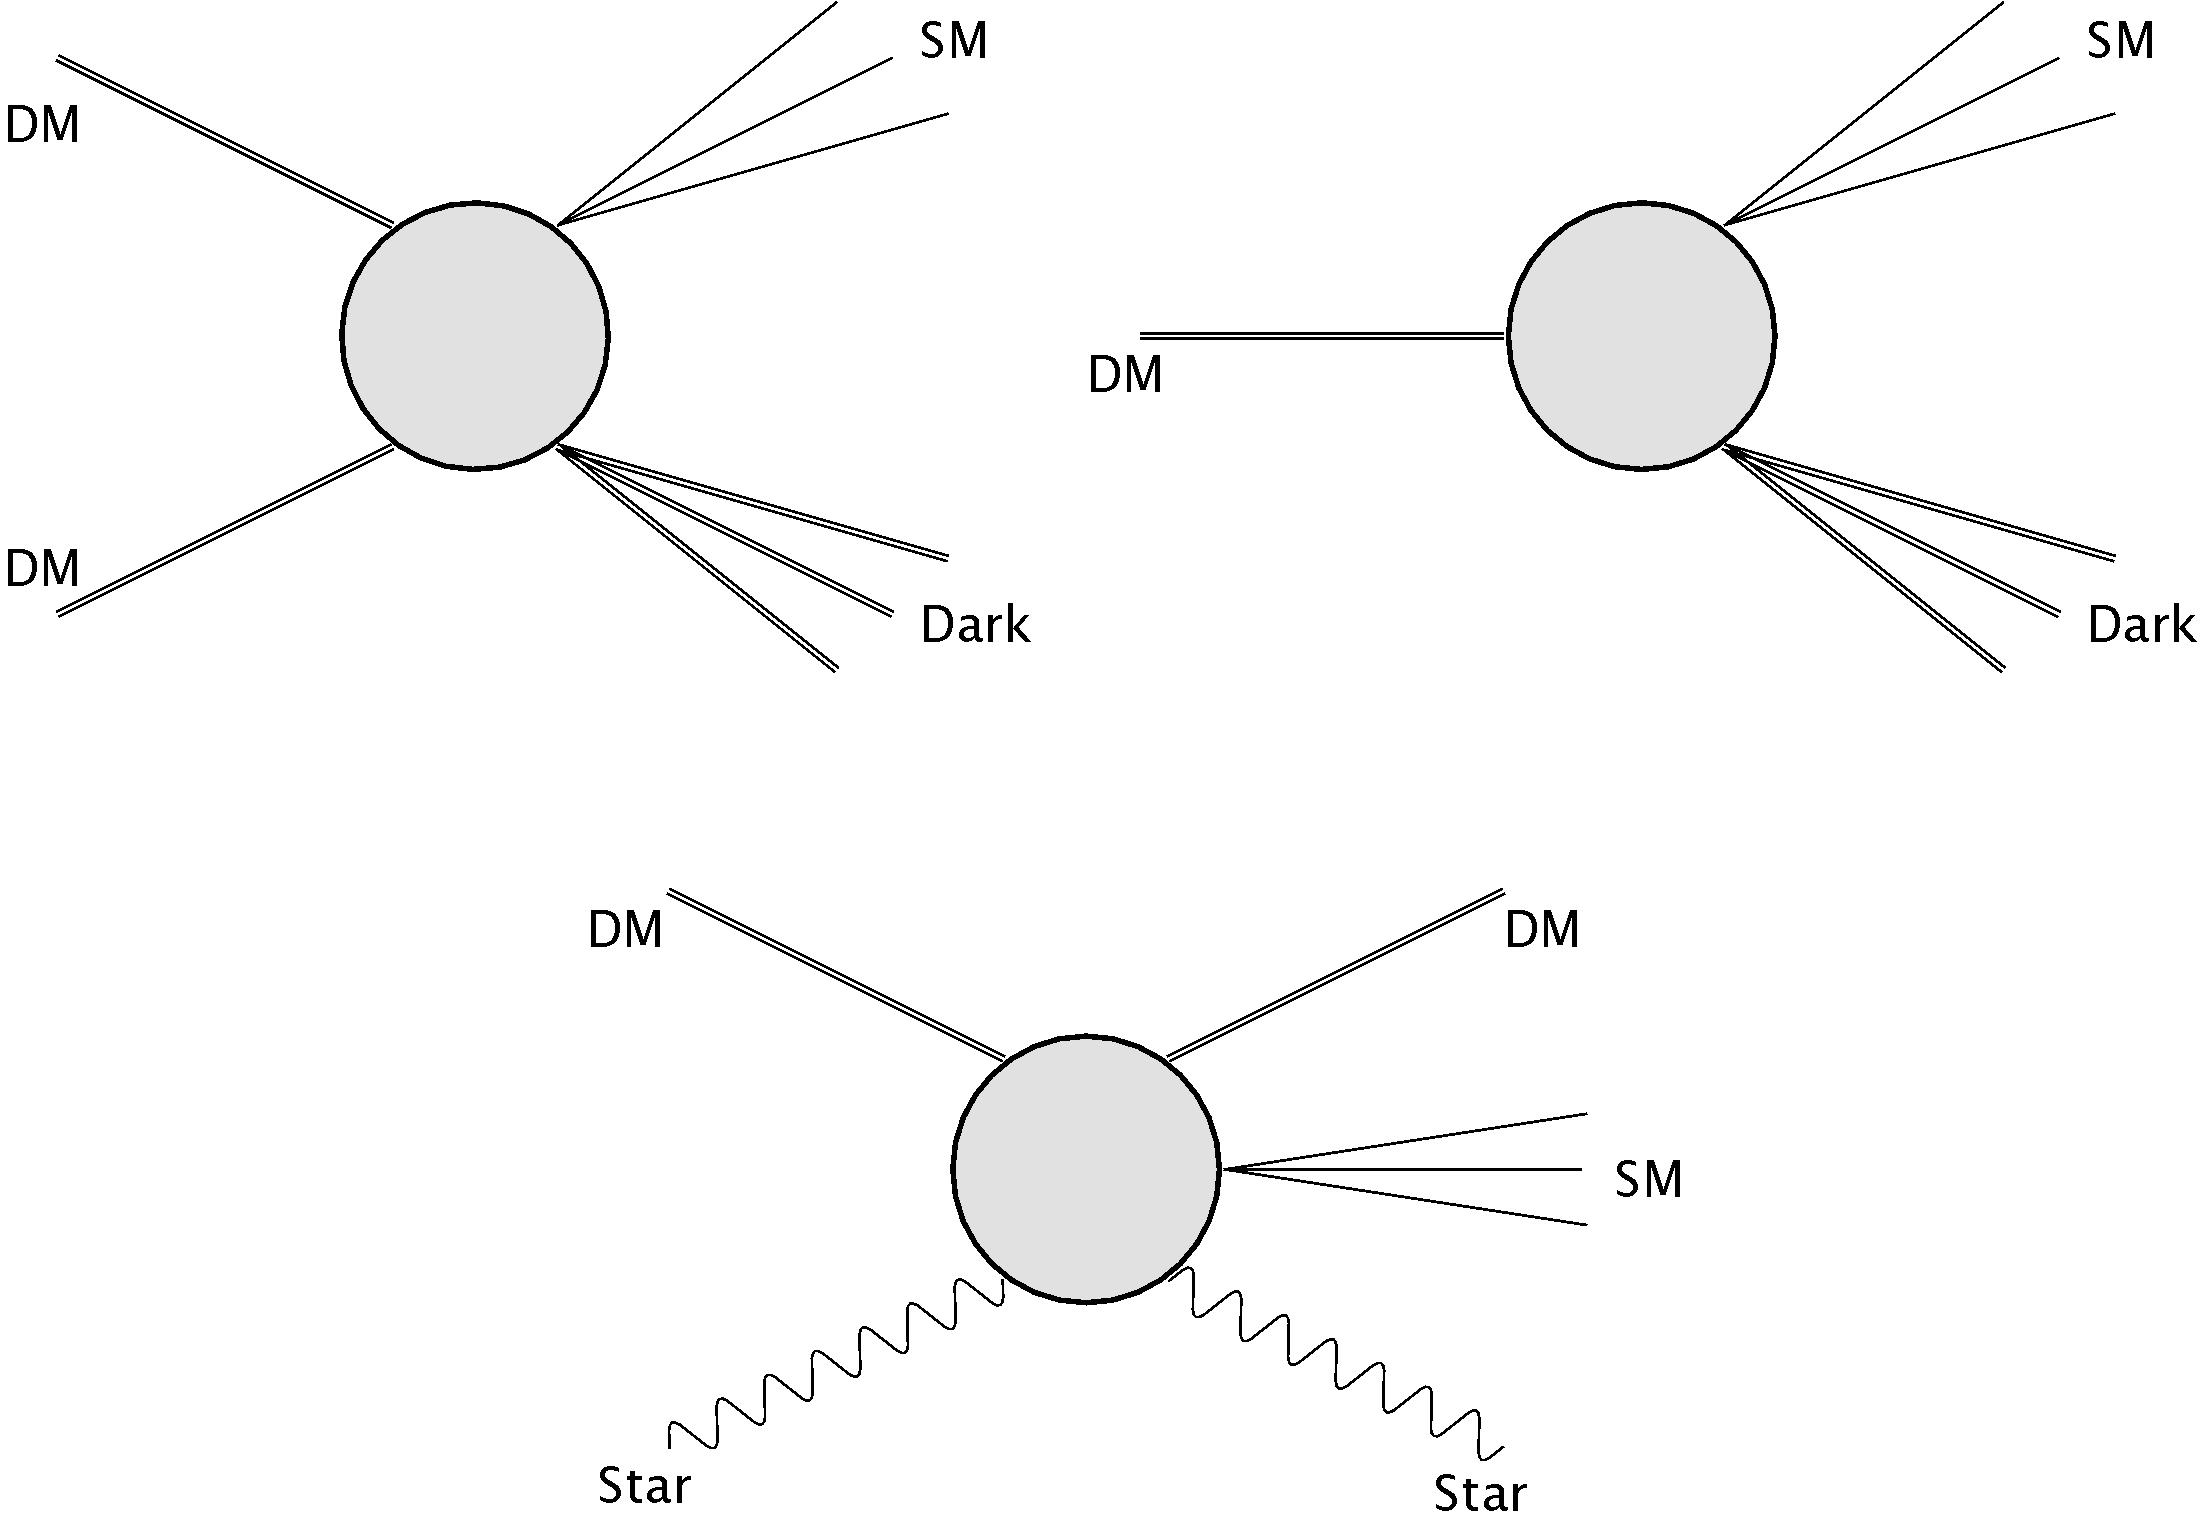
\includegraphics[scale=.05]{feynmandiag}
\caption{General interactions between ultra-heavy DM and WD constituents - \textcolor{blue}{do diagrams properly}}
\end{figure}

\subsection{DM Transit}

A DM transit releases energy continually along the DM trajectory, resulting in a cylindrical temperature profile of transverse length scale $L$, the heating length.  This $L$ is determined by the DM-SM interaction parameters and $n$.  Ignition will be determined by both $L$ and the amount of energy deposited per length along the DM trajectory, so we parameterize this interaction in terms of a (normalized) linear energy deposit $\chi_{led}$:
\[
    \chi_{led} =
    \frac{1}{n} \frac{\partial{E_{\text{led}}}}{\partial{x}}
\]
where $n$ is the number density of the stellar medium and $d{E}/d{x}$ is the kinetic energy deposited to the stellar medium per DM distance traveled.  Nominally, $\chi_{led}$ will depend on the stellar density $n$, the instantaneous DM energy $E$, and the details of the DM-SM interaction.  However, over the range of WD densities we consider it is reasonable that the only variation in $\partial E /\partial x$ for different stars is a linear scaling in $n$, so $\chi_{led}$ is independent of stellar variations.  \textcolor{red}{does this need more justification?} Further, all DM particles will enter the WD with speeds of order the escape velocity of the star, which is roughly a constant $v_{esc} \approx 10^{-2}$ for all WDs.  Thus the initial energy of a transiting DM particle depends only on its mass and so $\chi_{led}$ for a transit event is a function of only DM properties: $m_{DM}$ and its DM-SM interactions.

In order to ignite a WD during transit, the energy released must exceed the threshold \eqref{eq:boom}.  If the heating length $L > \lambda_T$, then we study one segment $L$ of the transit which behaves as a single energy deposit of length-scale $L$, as described in Section \ref{sec:review}. If $L < \lambda_T$, then over a $\lambda_T$ segment of the transit we have many $L$-scale heating events which sum to give a total energy deposited over the scale $\lambda_T$.  We consider thus the energy deposited in a transit of length $\text{max} \left\{ \lambda_T, L \right\}$, and requiring this to be greater than the threshold \eqref{eq:boom} we find a lower bound on the $\chi_{dep}$ sufficient to trigger runaway fusion:
\begin{equation}
\label{eq:transitexplosion}
  \chi_{led} \gtrsim T_f\, \text{max}\left\{ \lambda_T, L \right\}^2
\end{equation}

The validity of equation \eqref{eq:transitexplosion} requires two conditions.  First, in order for the deposited energy to to add coherently in forming an initial temperature profile, we need the DM transit time across the deposition region to be less than the thermal diffusion time across this region:
\begin{equation}
\tau_d \gtrsim \frac{\text{max}\left\{ \lambda_T, L \right\}}{v_\text{esc}},
\end{equation}
where the DM transit velocity is given by the WD escape velocity and $\tau_d$ is the characteristic time for a region of size $\text{max}\{\lambda_T, L\}$ and temperature $T_f$ to diffuse $\OO(1)$ of its thermal energy.  This scales as $\tau_d \sim \text{max}\left\{ \lambda_T, L \right\}^2/\alpha$, where $\alpha$ is the (temperature-dependent) diffusivity, so we require:
\begin{equation}
\alpha\left(T_f\right) \lesssim v_\text{esc} \text{max}\left\{ \lambda_T, L \right\} \label{eq:SlowDiffusion}
\end{equation}
This condition is independent of DM model, and is satisfied for all WD densities.
\textcolor{red}{Show this is actually true for all densities.} \textcolor{blue}{Also comment on $T \gg T_f$ (which only helps us? any other subtleties?)}

\textcolor{blue}{Similarly, we also require that the time to transfer energy $\epsilon$ out to the initial temperature profile of length $L$ is less than the diffusion time scale $\tau_d$.} \textcolor{red}{Is this necessarily a condition?}

Second, we have assumed that the DM particle does not slow down appreciable during the transit of the heating region, and more stringent, that it transits the star with the stellar escape speed.  Both of these are ensured by requiring that the DM-SM interaction is weak enough that the DM penetrates the non-degenerate crust of the WD unscathed. As only the degenerate interior is susceptible to runaway fusion, we must consider the energy deposit only after the crust is traversed and can thus ignore any variation in transit velocity only if the crust provides negligible energy loss.  This requires that we think about the stopping power of the DM, which is defined analogous to the linear energy deposit above but tracks instead the energy loss of the DM particle:
\begin{align}
\chi_{sp} = - \frac{1}{n} \frac{\partial{E_{\text{DM}}}}{\partial{x}}
\end{align}
For a crust size $R_{\text{c}}$ \textcolor{blue}{$\sim 50\, \text{km}$}, and conservatively assuming the crust density is $\OO(1)$ the interior density, we then require:
\begin{equation}
\frac{\chi_{sp}}{m_{DM}} \lesssim \frac{v_{esc}^2}{n R_c} \label{eq:Crust}
\end{equation}
\textcolor{blue}{assuming $\partial E_\text{DM}/\partial x$ is roughly constant\ldots}
Note that $\chi_{led}$ and $\chi_{sp}$ are not necessarily equal, though they will be in the important special case that the DM-SM interaction converts only DM kinetic energy into relativistic SM particles. We will consider this special case below, as well as an explicit model of Q-ball dark matter in which $\chi_{led} \gg \chi_{sp}$ .

It is important to note that if diffusion is too fast or the crust dramatically slows the DM, it is still possible to have an explosive transit event, but one would need to account for the additional diffusive cooling and slower transits. In this work, we will focus on events that satisfy conditions~\eqref{eq:SlowDiffusion} and~\eqref{eq:Crust} for simplicity.

{\color{red} Is the crust ``condition" a veto on explosiveness? probably not} 

{\color{blue}
Imposing \eqref{eq:transitexplosion}, we find lower bound on $m_{\text{DM}}$ such that the DM is able to both penetrate the crust \emph{and} trigger an explosion:
\begin{equation}
\label{eq:transitmass}
m_{\text{DM}} \gtrsim  T_f ~\text{max}\{\lambda_T, L\}^2 \l \frac{n_{\text{c}} R_{\text{c}}}{v_{\text{esc}}^2} \r
\end{equation}
If \eqref{eq:transitmass} is violated, then the DM interaction is either not strong enough to ignite the WD or it is so strong that it has no chance penetrate the crust and transit the interior. In the case of $\lambda_T > L$, this translates to a model-independent lower-bound on the DM mass $\sim 10^{27} - 10^{34} ~\GeV$. \textcolor{blue}{used 1 km crust and same number density as interior}.
}


\subsection{DM-DM Collisions}

\section{Heating Length}
\label{sec:HeatingLength}
For the DM interactions under consideration, the released energy must be efficiently transferred to the WD in order to trigger runaway fusion. In this section, we summarize the available modes of energy loss for different SM particles in a WD - detailed calculations of the various interactions are presented in Appendix \ref{sec:appendix}. For a given process, the heating length $L$ is approximately the distance over which an incident particle of energy $\epsilon$ and any secondaries deposit $\OO(1)$ of the initial energy \emph{and} the energy transfer thermalizes ions in the WD. As we are primarily concerned with depositing sufficient energy to ignite supernovae, we focus on high-energy particles $\epsilon \gg T_f \sim \text{MeV}$ which interact via the strong and electromagnetic forces: electrons, photons, muons, and hadrons. In this way, the WD may be thought of as a ``particle detector" with electromagnetic and hadronic ``calorimeter" components.

\subsection{Hadrons}
We primarily consider consider protons, neutrons, and pions. Although neutrons and $\pi^\pm$ decay through the weak interaction and have characteristically long lifetimes, the mean distance traversed by a neutral pion before decaying to photons $d_{\pi^0} = \gamma v \tau$ is of order $\lambda_T$ for pion energies less than $\sim \text{GeV}$.

The end products of a hadronic shower will generally be hadrons of kinetic energy $1-10 ~\text{MeV}$ which are incapable of inducing further cascades.

\subsection{Electrons and Photons}

\section{Constraints}
\label{sec:Constraints}

In this section, we constrain potential DM models following the discussion of \cite{Graham:2015apa} (1)~observation of white dwarfs that should have blown up already due to the presence of the candidate in sufficient abundance, and (2)~by observing a supernovae rate incompatible with the expected rate due to the DM candidate detonating WDs. We will consider each of these possibilities for both DM transits and collisions in the WD, but first we pause to consider the data available on white dwarfs and the supernovae rate.

\textcolor{blue}{Exhibit a specific white dwarf candidate and discuss its parameters: age, radius, mass (density), local dark matter density. Also mention possible white dwarf candidates in higher dark matter densities.}

\textcolor{blue}{Discuss the current supernovae rate and the attendant assumptions.}

\subsection{Dark Matter Transits}
\label{sec:TransitConstraints}

The expected number of ultra-heavy dark matter transits through a white dwarf with lifetime $t_\text{WD} \sim \text{Gyr}$ is given by
\begin{align}
N_\text{transits}  &= t_\text{WD} \cdot n_\text{DM} \sigma_g v \\
 &  \sim t_\text{WD} \cdot \frac{\rho_{\text{DM}}}{m_\text{DM}} \pi R_\text{WD}^2 \l\frac{v_\text{esc}}{v}\r^2 v,
\end{align}
where $v \sim 10^{-3}$ is the virial velocity of DM \textcolor{red}{(could be quite different near the galactic center with higher dark matter density?)} and $\rho_{\text{DM}}$ is the energy density of DM in the region of interest. $\sigma_g$ denotes the capture cross section including a gravitational Sommerfeld enhancement. Considering a $1.25 M_{\odot}$ WD in the local dark matter halo $\rho_{\text{DM}} \sim 0.3 ~\text{GeV}/\text{cm}^3$, we find that $m_\text{DM} \lesssim 10^{44} ~\GeV \sim 10^{20} ~\text{g}$ will transit the WD at least once in a Gyr. If we instead consider (recently discovered) heavy white dwarfs in the galactic center $\rho_{\text{DM}} \sim 10^3 ~\text{GeV}/\text{cm}^3$, this upper bound improves to $m_\text{DM} \lesssim 10^{48} ~\GeV \sim 10^{24} ~\text{g}$.

\textcolor{blue}{Considering these conditions, the independent parameters we are free to vary and constrain are the species $i$ released during a DM-SM collision, the energy $\epsilon$ released per particle, the weighted cross-section $N_i \epsilon\, \sigma_{\epsilon,i}$, the local mass density of the DM candidate $\rho_\text{DM}$, and the dark matter mass $m_\text{DM}$. The relevant heating length $L$ is then determined by $i$, $\epsilon$, and white dwarf parameters, and parameter constraints follow.}


\subsection{DM-DM Collisions}
\label{sec:CollisionConstraints}


\section{Concrete Examples}
\label{sec:ConcreteExamples}

The constraints developed in the previous section can be applied to a wide variety of ultra-heavy dark matter models. In the section we give two concrete examples to illustrate their application and to put new bounds on parameter space inaccessible to terrestrial experiments.

\subsection{Q-balls}
\label{sec:Qballs}
In various supersymmetric extensions of the standard model (SM), non-topological solitons called Q-balls can be produced in the early universe \cite{Coleman:1985ki, Kusenko:1997si}. If these Q-balls were stable, they would comprise a component of the dark matter today. In gauge-mediated models with flat scalar potentials, the Q-ball mass and radius are given by
\begin{equation}
\label{eq:Qballprop}
M_Q \sim m_F Q^{3/4}, ~~~ R_Q \sim m_F^{-1} Q^{1/4},
\end{equation}
where $m_F$ is related to the scale of supersymmetry breaking (messenger scale). The condition $M_Q/Q < m_p$ ensures that the Q-ball is stable against decay to nucleons \cite{Dine:2003ax}. When an (electrically neutral) baryonic Q-ball interacts with a nucleon, it absorbs its baryonic charge as a minimum-energy configuration and induces the dissociation of the nucleon into free quarks. During this process, $\sim \text{GeV}$ of energy is released through the emission of 2-3 pions \cite{Dine:2003ax}. The cross section for this interaction is approximately geometric:
\begin{equation}
\sigma_Q \simeq \pi R_Q^2.
\end{equation}
Note that a sufficiently massive Q-ball will become a black hole if the Q-ball radius is less than the Schwarzschild radius $R_Q \lesssim R_s \sim G M_Q$. In the model described above, this translates into a condition
\begin{equation}
m_F \l\frac{\Mpl}{m_F}\r^3 \lesssim m_Q, ~~~ \l\frac{\Mpl}{m_F}\r^4 \lesssim Q.
\end{equation}
For Q-ball masses of this order, gravitational interactions become relevant.

We assume that for each Q-ball collision, there is equal probability to produce $\pi^0, \pi^+$ and $\pi^-$ under the constraint of charge conservation, with average kinetic energy $\sim 500 ~\text{MeV}$. Numerous experiments have studied interactions of pions in this energy range incident upon complex nuclei targets such as carbon. It is found that there is roughly equal cross section of order $\OO (100 ~\text{mb})$ for a (neutral or charged) pion to either scatter elastically, scatter inelastically, or become absorbed with no final state pion \cite{Pionnuclear}. Of these possibilities, pion absorption is the most relevant for energy loss as this will induce a hadronic shower. Following the results of Section \ref{sec:heatinglength}, the relevant heating length $L$ of the Q-ball interaction is shown in 

Q-balls that transit a WD with sufficiently large cross section as given by \eqref{eq:transitexplosion} will ignite the star. The resulting explosive power for Q-balls is plotted in Figure \ref{fig:boomQball}. If the Q-ball cross section is related to its mass and baryonic charge as in \eqref{eq:Qballprop}, we find that
\begin{equation}
m_Q \gtrsim 10^8 ~\text{g} \l\frac{m_F}{\text{TeV}}\r^4, ~~~~ Q \gtrsim 10^{38} \l\frac{m_F}{\text{TeV}}\r^4
\end{equation}
is capable of triggering runaway fusion in a heavy $\sim 1.25 M_{\odot}$ WD.

\begin{figure}
\label{fig:boomQball}
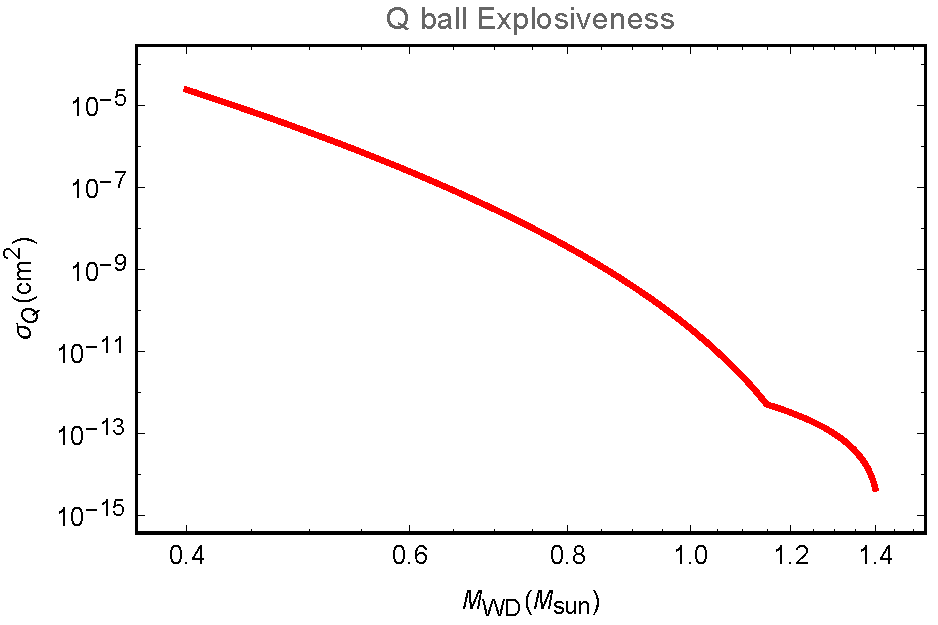
\includegraphics[scale=.45]{boomQball.pdf}
\end{figure}

\textcolor{blue}{Triangle Plot constraints of $Q - m_F$ on top of cosmic ray, Super-K bounds on Q balls}.

\section{Discussion}
\label{sec:discussion}

\begin{appendices}

\section{Particle Interactions in a White Dwarf}
\label{sec:appendix}

The interior of a WD is a complex environment (unless otherwise noted, we will assume a carbon-oxygen WD). Famously, the star is supported against collapse by electron degeneracy pressure with a characteristic Fermi energy
\begin{equation}
E_F = (3 \pi^2 n_e)^{1/3} \sim 0.1 - 1 ~\text{MeV}
\end{equation}
where $n_e$ is the number density of electrons. The nuclei are at an ambient temperature $T \sim \text{keV}$ and form a strongly-coupled plasma with coupling parameter
\begin{equation}
\Gamma \sim \frac{Z^2 \alpha}{n_i^{-1/3} T} \gg 1,
\end{equation}
where $n_i$ is the number density of nuclei. Here we provide a detailed analysis of the possible electromagnetic and strong interactions in a WD.

\subsection*{Coulomb Collisions}

An incident particle of mass $m$, charge $e$, and velocity $\beta$ scattering off a (stationary) target of mass $M$, charge $Ze$ with impact parameter $b$ will transfer energy
\begin{equation}
\label{eq:impact}
E' = \frac{2 Z^2 \alpha^2}{b^2 \beta ^2 M}.
\end{equation}
The differential cross section for the interaction is given by the Rutherford cross section
\begin{equation}
\label{eq:rutherford}
\frac{d \sigma_R}{dE'} = \frac{2 \pi  \alpha^2 Z^2}{M \beta^2} \frac{1}{E'^2},
 \end{equation}
where we have assumed a sufficiently fast incident particle so that interactions are governed by single collisions with energy transfer $E'$ \cite{Agashe:2014kda}.  Note that the differential cross section receives additional QED due to the incident spin, but for small energy transfers these corrections are negligible. It is straightforward to understand the parametric dependences of \eqref{eq:rutherford}: there is increased likelihood to scatter for slowly moving incident particles undergoing ``soft-scatters" against lighter targets. Therefore, one would expect that soft-scattering dominates the energy loss and that collisions with nuclei of mass $M$ are suppressed by a factor $\OO\l\frac{Z m_e}{M}\r$ as compared to collisions with electrons. This is certainly true for incident charged particles in non-degenerate matter. However, both of these naive expectations turn out to be false when considering scattering off a degenerate species.

We first consider the energy loss of high-energy charged particles colliding with non-degenerate targets. In this case, the stopping power is given by:
\begin{align}
\label{eq:SP}
-\frac{dE}{dx} & = - \int dE' \left(\frac{d \sigma}{dE'}\right) n E' \\
& \simeq -\frac{n_i \pi Z^2 \alpha^2}{M \beta^2} \log {\l\frac{E_{\text{max}}}{E_{\text{min}}}\r}.
\end{align}
\eqref{eq:SP} must be integrated over all $E'$ within the regime of validity for \eqref{eq:rutherford}, thereby fixing the lower and upper bounds of the Coulomb logarithm. The maximum possible energy transfer satisfying kinematic constraints in a backward scatter is given by
\begin{equation}
E_{\text{kin}} = \frac{2 M \beta^2 \gamma^2}{1+ 2\gamma M/m +(M/m)^2},
\end{equation}
where $\gamma = (1-\beta^2)^{-1/2}$ is the relativistic factor. In addition, quantum mechanical uncertainty sets a limit to the accuracy that can be achieved in ``aiming" an incident particle at a target $b > \frac{1}{\text{min}\{{M, m}\} \beta \gamma}$. In terms of energy transfer, this translates to the condition
\begin{equation}
E' < E_\text{quant} = \frac{2 Z^2 \alpha^2 \gamma^2 ~\text{min}\{{M, m}\}^2}{M}.
\end{equation}
Furthermore, the expression for the energy loss in a scatter \eqref{eq:impact} is modified by relativistic considerations when the energy transfer is larger than the target mass \cite{Rossi}. For our purposes, we take the maximum energy that an incident particle is able to transfer to be
\begin{equation}
E_{\text{max}} = \text{min}\{E_\text{quant}, E_{\text{kin}}, M\}.
\end{equation}

On the other hand, the maximum impact parameter is set by Thomas-Fermi screening due to the degenerate electron gas:
\begin{equation}
\label{eq:TF}
\lambda_{\text{TF}} = \l \frac{6 \pi Z \alpha n_e}{E_F}\r^{-1/2}.
\end{equation}
This corresponds to a lower bound on the energy transfer
\begin{equation}
E' > E_{\text{sc}} = \frac{12 \pi Z^3 \alpha ^3 n_e}{\beta^2 M E_F}.
\end{equation}
In addition, the lattice structure of ions in the WD introduces further complications \cite{Teukolsky}. The typical Coulomb lattice binding energy between ions is given by the electric potential
\begin{equation}
\label{eq:lattice}
E_B \sim \frac{Z^2 \alpha}{n_i^{-1/3}} \sim 10^{-2} - 10^{-1} ~\text{MeV}
\end{equation}
For energy transfers greater than $E_B$, lattice effects can be safely ignored. On the other hand, momentum transfers from collisions below this threshold will lead to suppressed energy loss due to collective effects (i.e. phonon excitations) For simplicity, we set the lower bound on nuclei scattering (not applicable for electron targets) to be
\begin{equation}
E_{\text{min}} = \text{max} \{E_B,E_{\text{sc}}\}
\end{equation}
so that we only account for energy transfers greater than the ion lattice binding energy.

Now consider collisions with degenerate electrons. An incident particle transferring energy $E'$ can only scatter those electrons within $E'$ of the Fermi surface. We define a modified density of electrons $n_e(E')$ as:
\begin{equation}
\label{pauli}
n_e(E') = \left\{
        \begin{array}{ll}
            \displaystyle \int \limits_{E_F -E'}^{E_F}dE ~g(E) & \quad E_F \geq E' \\
            n_e & \quad E_F \leq E'
        \end{array}
    \right.,
\end{equation}
where $g(E)$ is the density of states per unit volume for a three-dimensional free electron gas. The effect of degeneracy can also be cast as a suppression of the differential cross section of order $\mathcal{O}(E'/E_F)$ whenever energy less than the Fermi energy is transferred. Therefore, unlike in the non-degenerate case, the energy loss due to soft-scatters are in fact \emph{subdominant} to the contributions from rare hard-scatters. The stopping power is also sensitive to the integration bounds $E_{\text{max}}$ and $E_{\text{min}}$ as a power-law dependence unlike the logarithmic sensitivity \eqref{eq:SP} in the case of a non-degenerate target.

\subsection*{Compton Scattering}
High-energy photons can efficiently deposit their energy to electrons in the WD via Compton scattering
\begin{equation}
{k^{\prime }={\frac {k}{1+{\frac {k}{m_{\text{e}}c^{2}}}(1-\cos \theta )}}},
\end{equation}
where $k$ and $\theta$ denote the energy and angle of deflection for the incident photon, respectively. For perfectly forward scatters, none of the initial energy is transferred while for energetic photons $k \gg m_e$, the maximal energy transfer approaches the initial energy. The differential cross section for photons to scatter off a free electron is given by the Klein-Nishina formula:
\begin{equation}
\label{KN}
\frac{d\sigma_\text{KN}}{d (\cos \theta)}=\frac{\pi \alpha^2}{m_e^2} \l \frac{k'}{k} + \frac{k}{k'} -\sin^2 \theta \r.
\end{equation}

The stopping power due to Compton scattering can be expressed in terms of \eqref{KN}
\begin{equation}
\frac{dE}{dx} =  \int d (\cos \theta) n_e \frac{d\sigma_\text{KN}}{d (\cos \theta)} E', ~~~ E' = k - k'.
\end{equation}
Degeneracy can also be taken into account using a variable number density as in \eqref{pauli}, although this only introduces a significant suppression of the Compton stopping power for $k\lesssim 10 ~\text{MeV}$. 

\textcolor{blue}{Inverse Compton?}

\subsection*{Bremsstrahlung and Pair Production}
The cross section for an electron of energy $E$ to radiate a photon of energy $k$ in a medium with nuclear density $n$ is given by the Bethe-Heitler formula
\begin{equation}
\label{eq:BH}
\frac{d \sigma_\text{BH}}{dk} = \frac{1}{3 k n X_0} (y^2+2 [1+ (1-y)^2]), ~~~ y = k/E.
\end{equation}
$X_0$ is the radiation length, and is generally of the form
\begin{equation}
X_0^{-1} = 4 n Z^2 \frac{\alpha^3}{m_e^2} \log{\Lambda}, ~~~ \log{\Lambda} \sim \int \limits_{b_\text{min}}^{b_\text{max}} \frac{1}{b}.
\end{equation}
where $\log{\Lambda}$ is a logarithmic form factor containing the maximum and minimum effective impact parameters allowed in the scatter. $b_\text{min}$ is set by a quantum-mechanical bound such that the radiated photon frequency is not larger than the initial electron energy. For a bare nucleus, this distance is the electron Compton wavelength $b_\text{min} = \lambda_e = \frac{1}{m_e}$. It is important to note that collisions at impact parameters \emph{less} than $b_\text{min}$ will still radiate, but with exponentially suppressed intensity. Classically, this is manifested by the decoherence of radiation at large scattering angles. $b_\text{max}$ is set by the distance at which the nuclear target is screened. For an atomic target this is of order the Bohr radius, and in the WD this is the Thomas-Fermi length \eqref{eq:TF}. Immediately it is evident that there exists a critical number density at which $\log \Lambda \to 0$. Roughly this occurs at an electron number density $\sim 10^{32} ~\text{cm}^{-3}$. In a dense WD medium, the bremsstrahlung amplitude will be highly suppressed. We simply take $\log{\Lambda} \sim \OO(1)$ whenever $b_\text{min} \lesssim b_\text{max}$.

Similar to \eqref{eq:BH}, the cross section for a photon of energy $k$ to produce an electron-positron pair with energies $E$ and $k-E$ is
\begin{equation}
\label{eq:PP}
\frac{d \sigma_\text{BH}}{dE} = \frac{1}{3 k n X_0} (1+ 2[x^2+ (1-x)^2]), ~~~ x = E/k.
\end{equation}
Note that pair production has a threshold energy so that \eqref{eq:PP} is only valid for $k \gtrsim m_e$. Integrating \eqref{eq:BH}, the energy loss due to bremsstrahlung is simply
\begin{equation}
\frac{dE}{dx} = \frac{E}{X_0},
\end{equation}
and the full pair production cross section is $\sigma_{pp} = \frac{7}{9} \frac{1}{n X_0}$. In effect, $X_0$ is the typical length scale of an electromagnetic shower.

However, bremsstrahlung and pair production will be suppressed by the ``Landau-Pomeranchuk-Migdal" (LPM) effect (see \cite{Klein:1998du} for an extensive review). High-energy radiative processes involve very small longitudinal momentum transfers to nuclear targets ($\propto k/E^2$ in the case of bremsstrahlung). Quantum mechanically, this interaction is delocalized across a formation length over which amplitudes from different scattering centers will interfere. This interference is usually destructive and must be taken into account in the case of high energies or high-density mediums. Calculations of the LPM effect can be done semi-classically based on average multiple scattering. It is found that bremsstrahlung is suppressed for $k > E(E-k)/E_\text{LPM}$ and pair production for $E(k-E) > k E_\text{LPM}$, where
\begin{equation}
\label{eq:LPM}
E_\text{LPM} = \frac{m_e^2 X_0 \alpha}{4 \pi}.
\end{equation}
For the WD densities under consideration, $E_\text{LPM} \sim 10-10^{3} ~\text{MeV}$. With LPM suppression, the bremsstrahlung stopping power is approximately
\begin{equation}
\label{eq:bremloss}
\l\frac{dE}{dx}\r_\text{LPM} \sim \l\frac{E_\text{LPM}}{E} \r^{1/2} \frac{E}{X_0}, ~~~ E>E_\text{LPM}.
\end{equation}
We find that the LPM effect diminishes the energy loss due to soft radiation so that the radiative stopping power is dominated by single, hard bremsstrahlung. Similarly, the pair production cross section reduces to
\begin{equation}
\sigma_{pp} \sim \l\frac{E_\text{LPM}}{k} \r^{1/2} \frac{1}{n X_0}, ~~~ E>E_\text{LPM}
\end{equation}

In addition to multiple scattering, additional interactions within a formation length will suppress bremsstrahlung when $k \ll E$. The emitted photon can coherently scatter off electrons and ions in the media, acquiring an effective mass of order the plasma frequency $\omega_p$. The fastest plasma frequency will dominate, which is set by degenerate electrons.
Semi-classically, this results in a suppression of order $(k m_e/\omega_p E)^2$ when the radiated photon energy $k < \omega_p E/m_e$. This is known as the ``dielectric effect". Note that for the densities in question, $\omega_p < m_e$ so for our purposes, we may simply set $\omega E/m_e$ as a minimum cutoff on allowed photon frequencies. For high-energy electrons, this dielectric suppression only introduces a minor correction to \eqref{eq:bremloss}, in which soft radiation is already suppressed by the LPM effect \cite{Klein:1998du}. 

When bremsstrahlung is sufficiently suppressed, higher-order processes such as direct pair production $e N \rightarrow e^+ e^- e N$ should also be considered. The electron energy loss due to direct pair production has been computed in \cite{Gerhardt:2010bj} taking the LPM effect into consideration, although other possible diagrams have not been computed in the same manner. For our purposes, we ignore bremsstrahlung and pair production once the LPM suppression exceeds $\OO(\alpha)$. 

\subsection*{Nuclear Interactions}
Nuclear interactions can be either elastic or nonelastic - the nature of the interaction is largely determined by the incident particle energy. Elastic collisions are most relevant at scales less than the nuclear binding energy $E_\text{nuc} \sim 10 ~\text{MeV}$. A single, backward elastic scatter would result in an incident particle losing virtually all of its energy if the incident and target masses are the same. However, we will be primarily concerned with light hadrons incident on relatively heavy nuclei, i.e. ping-pong balls bouncing around a sea of bowling balls.
An elastic collision between an incident (non-relativistic) mass $m$ and a heavy, stationary target mass $M$ results in a final energy
\begin{equation}
\label{eq:elasticratio}
\zeta \equiv \frac{E_f}{E_0} \approx \l \frac{M}{M+m} \r^2, ~~~~ m < M.
\end{equation}
$E_0$ and $E_f$ denote the initial and final energy of the incident particle, and we assume an isotropic distribution in the center-of-mass scattering angle. Thus, a nucleon interacting with carbon nuclei transfers roughly 15\% of its incident energy after each elastic collision.

The cross section for elastic scatters has considerable dependence on the incident particle species. At energies below $\sim \text{MeV}$, the elastic cross section effectively vanishes for  protons. This can be understood physically as a strong interaction may only occur if an incident energy is sufficient to overcome the mutual Coulomb repulsion. For neutrons, the cross section is roughly constant below $\sim \text{MeV}$ but in the intermediate regime $1 ~\text{MeV} - \text{10} ~\text{MeV}$ is of a complicated form due to various nuclear resonances \textcolor{blue}{see evaluated nuclear data file}. For simplicity, we assume the elastic cross section for any hadron in this range to be a constant $\sigma_\text{el} \approx 0.1 ~\text{mb}$. Note that the neutron capture cross section in C and O nuclei is negligible compared to the elastic cross section in this energy range. However, since the ions in a WD form a Coulomb lattice, elastic collisions cannot transfer energy less than \eqref{eq:lattice} without exciting additional phonon modes. This limits the applicability of \eqref{eq:elasticratio} to energies above $\sim \text{MeV}$.

Next we consider nonelastic collisions, which are only possible at incident energies $\sim E_\text{nuc}$. In this regime, a nuclear collision generally results in an $\OO(1)$ number of energetic secondary hadrons (i.e. protons, neutrons, pions, etc.) emitted roughly in the direction of the primary particle. These secondary particles approximately split the initial total energy of the absorbed primary particle and can collide with other nuclei in the WD. The remnant nucleus will generally be left in an excited state and relax through the emission of $\OO(10 ~\text{MeV})$ hadrons (``nuclear evaporation") and photons \cite{Rossi}. A hadronic shower is the result of all such reactions caused by primary and secondary particles.

For simplicity, we take the nuclear mean free path for a light hadron (proton, neutron, pion) to be constant in energy with characteristic cross section
\begin{equation}
l_\text{had} \sim  \frac{1}{n_i \sigma_\text{non}}, ~~~~ \sigma_\text{non} \sim 100 ~\text{mb}.
\end{equation}
Note that the shower length is only logarithmically sensitive to the initial energy or number of secondaries, and is thus primarily set by the nuclear mean free path. In this case, the cascade induced by a high-energy initial hadron is adequately described by a stopping power
\begin{equation}
\label{eq:nucshower}
\l \frac{dE}{dx}\r_\text{had} \sim \frac{E}{l_\text{had}},
\end{equation}
neglecting logarithmic factors of $\OO(1)$. The shower will end once final-state hadrons reach a critical energy $E_c$ - this is either set by the scale at which an additional mechanism dominates the stopping power or the minimum energy required to induce further showers $E_\text{nuc}$. In this model, the total hadronic shower length $X_{\text{had}}$ for an incident hadron of energy $E_0 \gtrsim 10 ~\text{MeV}$ is given by
\begin{equation}
X_{\text{had}} \sim l_\text{had} \log{(E_0/E_c)} \approx 10 ~l_\text{had}.
\end{equation}

Energetic $k \gtrsim 10 ~\text{MeV}$ photons can also interact with nuclei and induce a hadronic shower. There is considerable uncertainty in the evaluation of high-energy photonuclear cross sections, and a detailed model is beyond the scope of this work. As a conservative estimate, \textcolor{blue}{we assume a constant value}
\begin{equation}
l_\gamma \sim \frac{1}{n_i \sigma_{\gamma A}}, ~~~~ \sigma_{\gamma A} \sim 1 ~\text{mb}.
\end{equation}

At ultra-high energies $k \gtrsim \textcolor{blue}{something}$ photonuclear interactions can become coherent, with the photon interaction spread over multiple nuclei \cite{Agashe:2014kda}. Similarly, charged leptons will lose energy via electronuclear interactions in which the incident particle radiates a virtual photon that then interacts hadronically with a nearby nucleus. Note that a hadronic shower induced by electronuclear interactions are not affected by the LPM suppression \eqref{eq:LPM}. Naively we expect the stopping power to be of order $\sim E \alpha/l_\gamma$. A more detailed calculation \cite{Gerhardt:2010bj} differs from our naive estimate an $\OO(10)$ factor. The largest uncertainty in calculating electronuclear stopping power at high energies is in evaluating hadronic cross sections, which require significant extrapolation from existing data and for which different models yield different results.

\end{appendices}

\section*{Acknowledgements}
We are grateful to S. Rajendran for suggesting this project and for helpful conversations. We would also like to thank D. Grabowska, K. Harigaya, S.R. Klein, R. McGehee, and J. Wurtele for stimulating discussions.

\bibliography{Qballs}

\end{document}
